Our pilot study reveals that hallucination detection method performance varies dramatically across benchmarks.

\subsection{Main Results}

\begin{table}[h]
\centering
\begin{tabular}{@{}lcc@{}}
\toprule
\textbf{Method} & \textbf{TruthfulQA} & \textbf{HaluEval} \\
\midrule
Semantic Entropy & 0.289 [0.105, 0.526] & \textbf{0.551} [0.267, 0.800] \\
Self-Consistency & 0.474 [0.252, 0.687] & 0.444 [0.155, 0.733] \\
\midrule
\emph{Gate Threshold} & \emph{0.55} & \emph{0.55} \\
\bottomrule
\end{tabular}
\caption{Hallucination Detection AUROC (Pilot Study, $N=20$ samples per dataset). Confidence intervals are 95\% bootstrap intervals.}
\label{tab:results}
\end{table}

\textbf{Key Observations:}

\begin{enumerate}
    \item \textbf{Only one condition meets the gate threshold.} Semantic entropy achieves AUROC 0.551 on HaluEval, marginally exceeding our 0.55 threshold.

    \item \textbf{TruthfulQA shows inverted results for semantic entropy.} AUROC 0.289 is below random (0.5), indicating high-entropy responses were actually more truthful.

    \item \textbf{Self-consistency performs near random on both benchmarks.} AUROC values of 0.444 and 0.474 are statistically indistinguishable from chance.
\end{enumerate}

\subsection{Benchmark Sensitivity Analysis}

Method ranking differs across benchmarks: semantic entropy outperforms self-consistency on HaluEval (0.551 vs 0.444), but the pattern reverses on TruthfulQA (0.289 vs 0.474). This interaction suggests benchmark-specific method selection may be necessary.

\subsection{Gate Evaluation}

\textbf{Gate Result:} PARTIAL (1/4 conditions pass)

\begin{table}[h]
\centering
\begin{tabular}{@{}lcc@{}}
\toprule
\textbf{Method} & \textbf{TruthfulQA} & \textbf{HaluEval} \\
\midrule
Semantic Entropy & FAIL & PASS \\
Self-Consistency & FAIL & FAIL \\
\bottomrule
\end{tabular}
\caption{Gate evaluation summary.}
\label{tab:gate}
\end{table}

\begin{figure}[h]
\centering
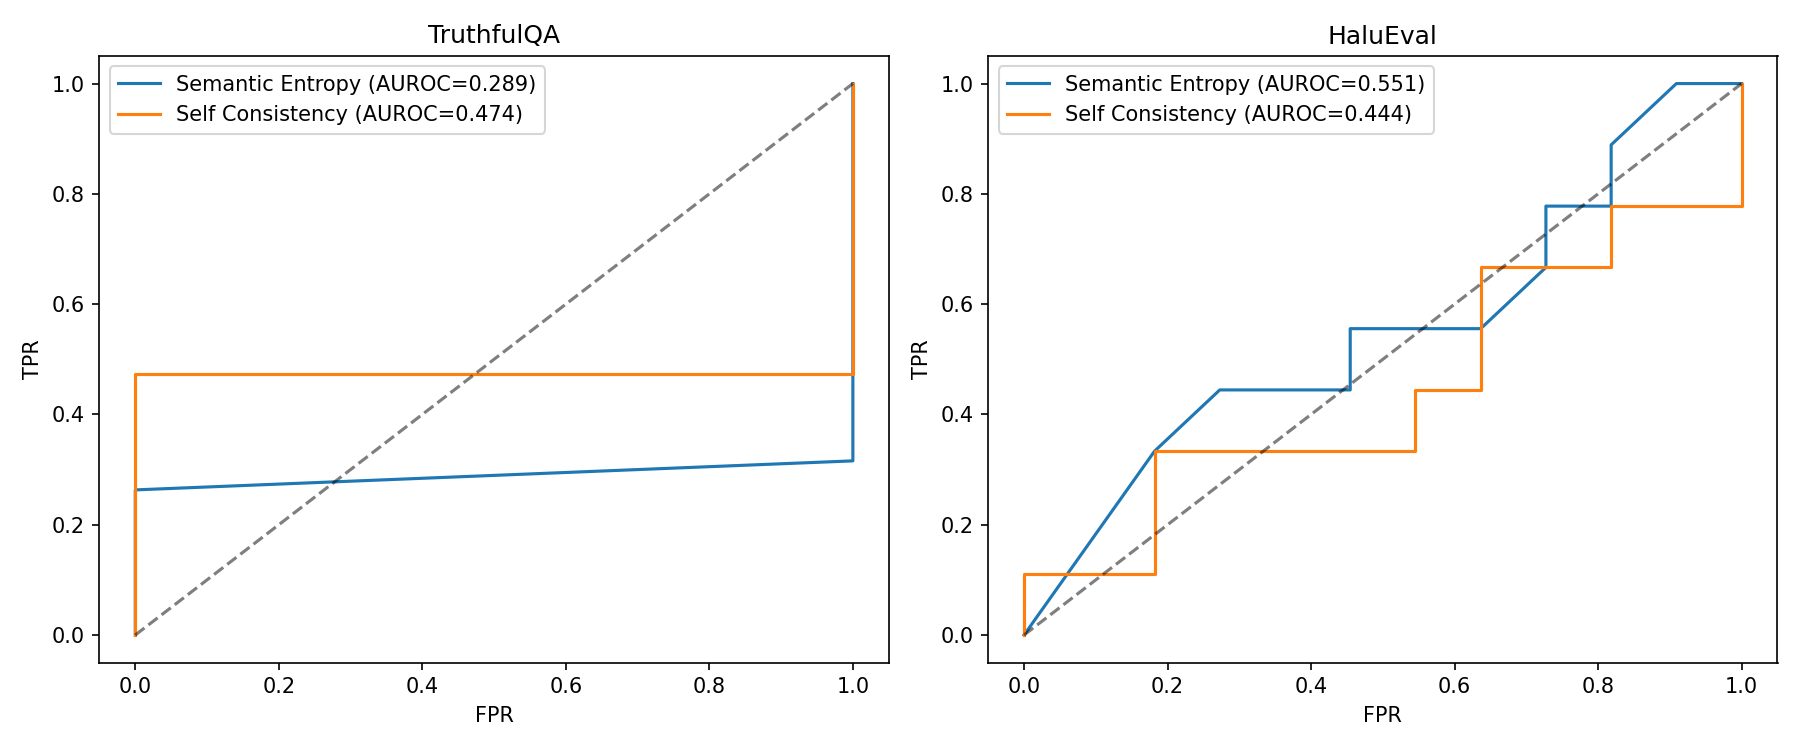
\includegraphics[width=0.8\columnwidth]{figures/roc_curves.png}
\caption{ROC curves comparing detection methods across benchmarks.}
\label{fig:roc}
\end{figure}

\begin{figure}[h]
\centering
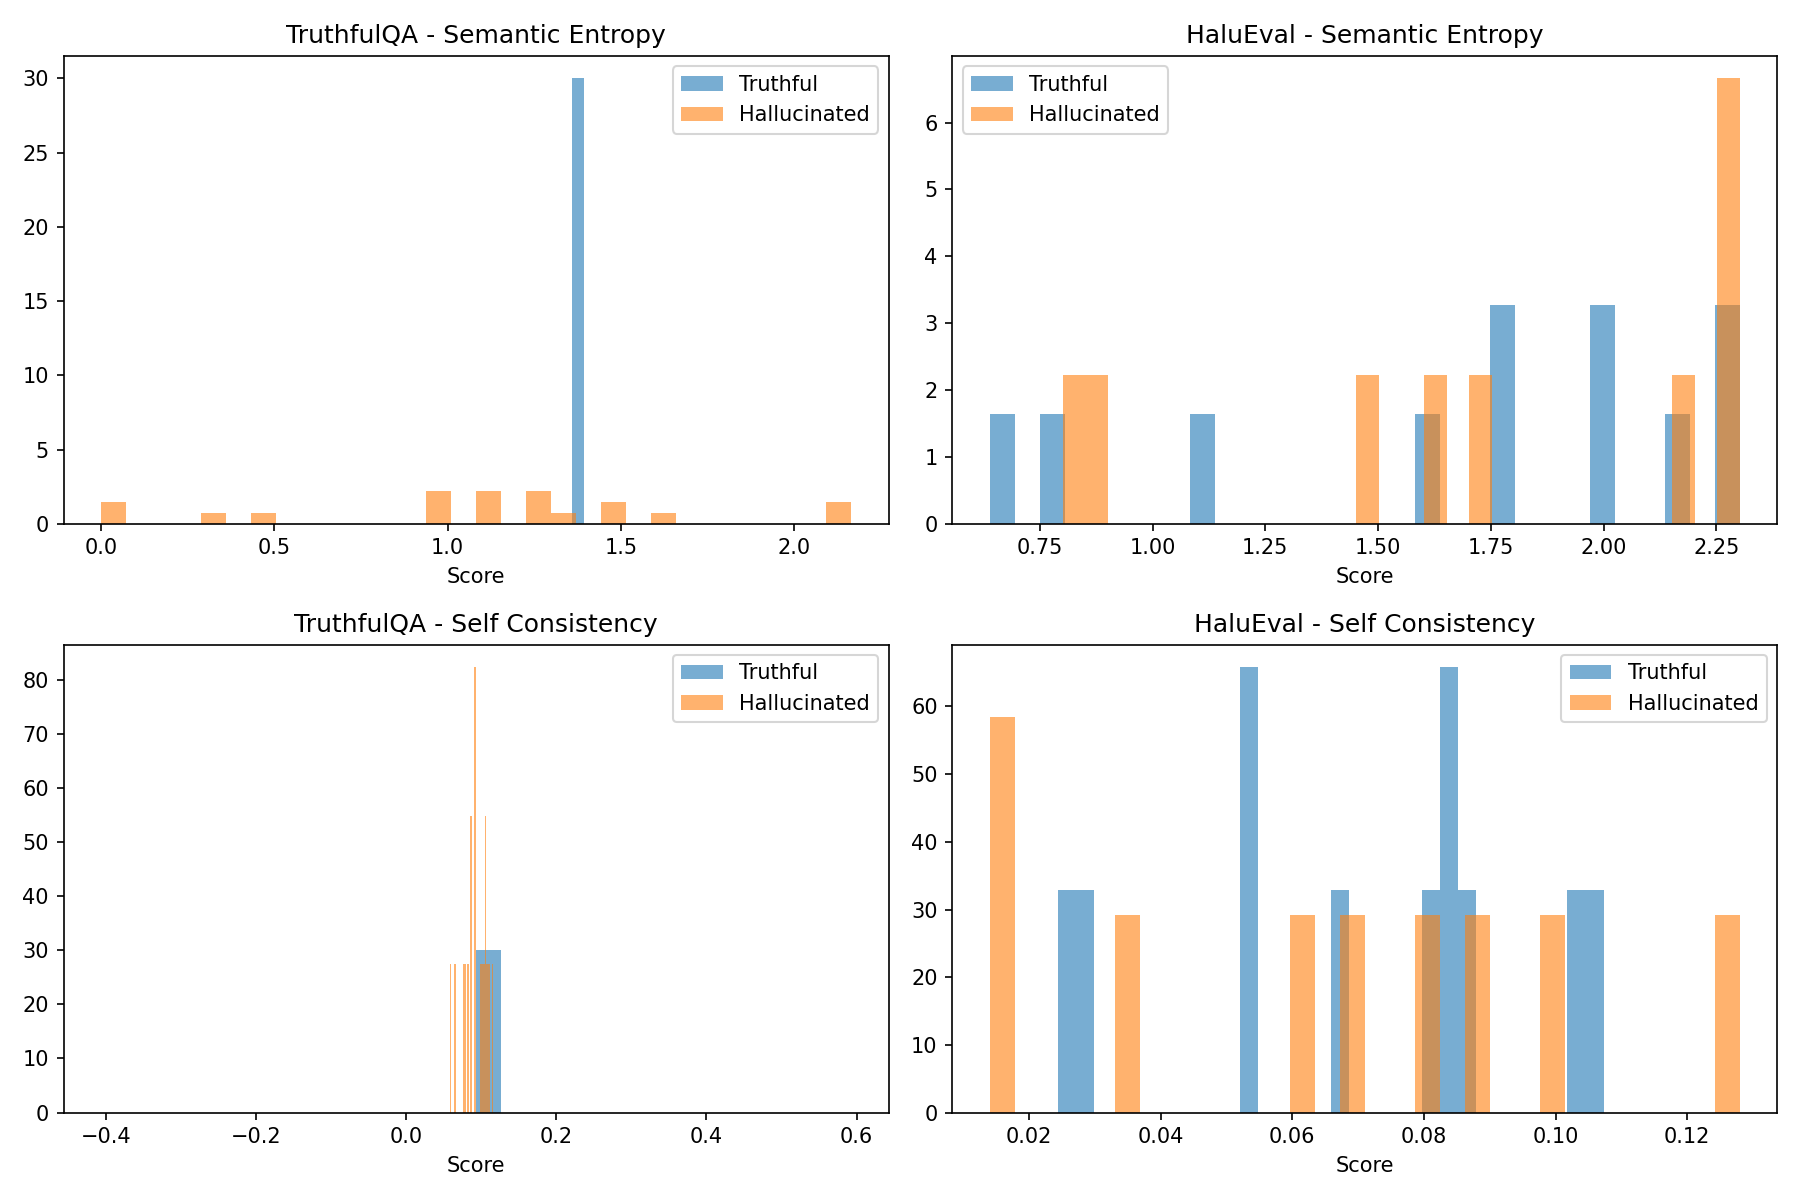
\includegraphics[width=0.8\columnwidth]{figures/score_distributions.png}
\caption{Distribution of uncertainty scores for hallucinated vs truthful responses.}
\label{fig:distributions}
\end{figure}

\begin{figure}[h]
\centering
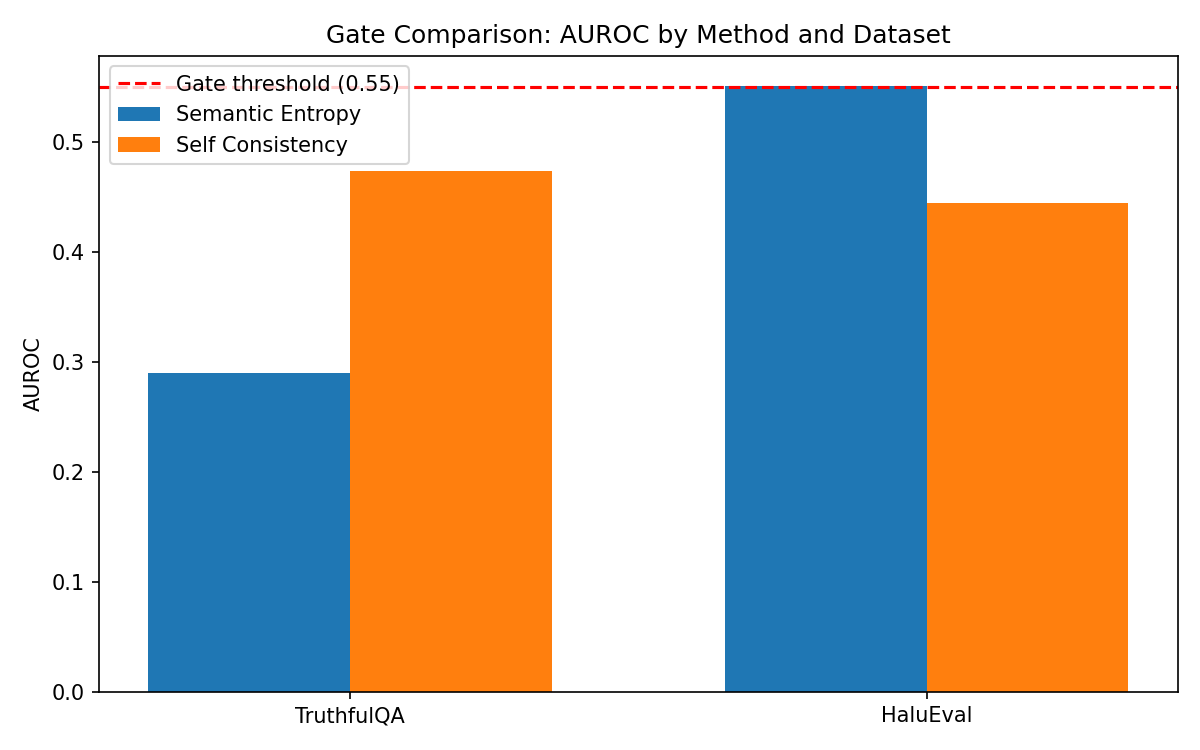
\includegraphics[width=0.8\columnwidth]{figures/gate_comparison.png}
\caption{AUROC comparison against 0.55 gate threshold.}
\label{fig:gate}
\end{figure}
